% !TEX root = summary-ipcv.tex
\section{Repetition SW01}
\itemsep0pt
\item \textbf{Histogramme} stellen die Häufigkeit der Farbverteilung dar.
\item \textbf{Hisogram-Ausggleich} stellt sicher, dass die Farbverteilung gleichmässig ist. Der Kontrast wird da verstärkt wo Glockenkurve hoch ist. Diese wird beim Ausgleich breiter. Führt zu mehr Kontraste.
\item \textbf{Punktbildfunktionen} brechnen ausgehend von einem alten Wert ein neuer Farb/Grauwert.
\item \textbf{Morphologische Operationen} werden auf binären Bilder angewendet. 
Dilate/Erode und Opening/Closing sind entsprechende Operationen. Kann für Zähöungen verwendet werden. Bei Morpholigische Operationen ist Vordergrund immer weiss, das bedeutet, dass bei einem Bild mit weissem Hintergrund das Bild invertiert werden soll.
\section{Farben}


\subsubsection{Farbe}
\begin{itemize}
	\itemsep0pt
	\item \textbf{Eine Farbe} ist eine elektromagnetische Strahlung in einer bestimmten Frequenz. Viele Farbsysteme haben nur drei Kanäle, weil der Mensch auch nur drei Arten von Zäpfchen haben. Es gibt verschiedene Spektren von Lichtquellen um Farben darzustellen. Zum Beispiel ergibt das ganze Spektrum von Sonnenlicht die Farbe weiss. Oder Quecksilber (Mercury) alle vier zusammen ergibt auch weiss
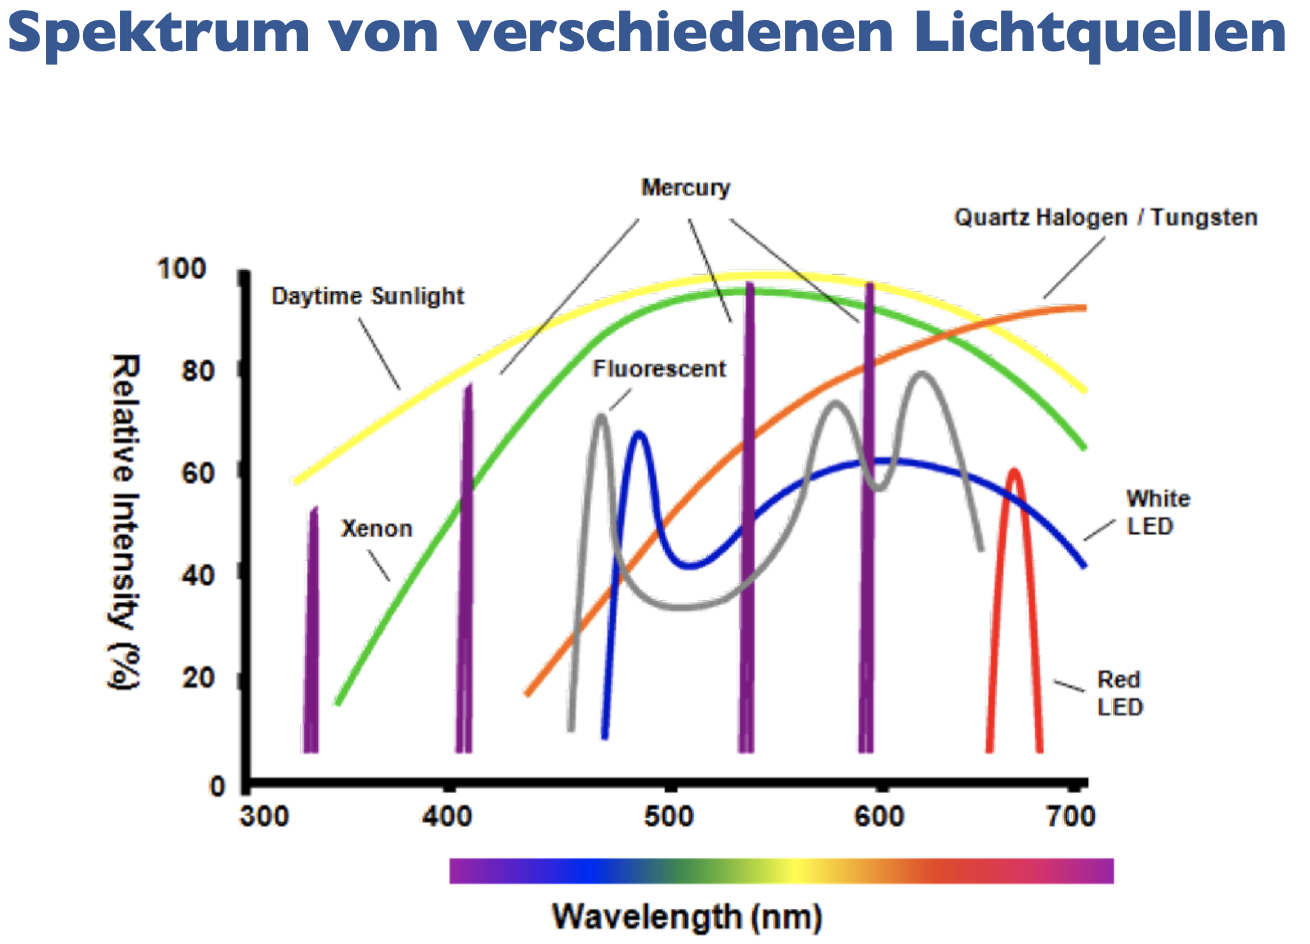
\includegraphics{images/sw02/spektrum-lichtquellen.png} 
	\item \textbf{Bildverarbeitung:} Erkennung von Objekten oder Szenen aus Bildern.
\end{itemize}

\subsubsection{Bildverarbeitung auf verschiedenen Stufen}
\begin{center}
	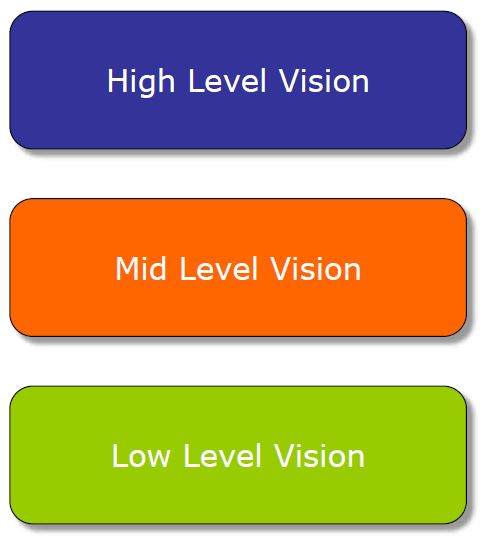
\includegraphics[height=3cm,keepaspectratio]{images/sw01/StufenBildverarbeitung.JPG}
\end{center}

\begin{itemize}
	\itemsep0pt
	\item Computer Vision (High Level Vision): Interpretation des Bildes, Erkennung von Objekten. 
	\item Image Processing (Low Level Vision): Bildverbesserung (Kontrastkorrektur, Rauschunterdrückung), Erkennung von Low Level Features (Kanten, Linien,...)
\end{itemize}

